\subsection{Recopilaci\'on de datos del software y desempe\~no 1}
    La recopilaci\'on de datos sobre el software y desempe\~no
        fueron basadas en distintas configuraciones iniciales, las
        cuales fueron introducidas en el simulador como la
        condici\'on inicial de la simulaci\'on. Estas pruebas fueron,
        adem\'as, recopiladas tanto en el sistema operativo de
        Windows como el de Linux, que son las dos plataformas en
        las cuales el programa puede funcionar. Los datos
        recopilados se muestran de las Figuras \ref{fig:Ruta 6} - \ref{fig:Ruta 16}.
    \vskip 0.5cm
    %figura
    \begin{figure}[htbp]
        \centering
        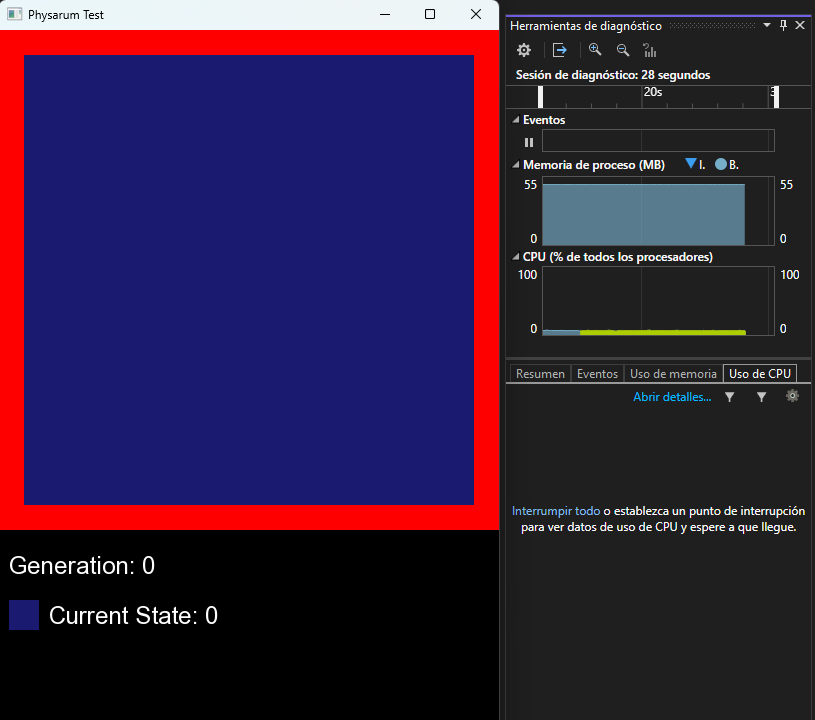
\includegraphics[width=0.5\textwidth]{./images/Pruebas/simulador/image019.png}
        \caption{Rendimiento de la aplicaci\'on sin estados adicionales en Windows}
        \label{fig:Ruta 6}
    \end{figure}
    \vskip 0.5cm
    %figura
    \begin{figure}[htbp]
        \centering
        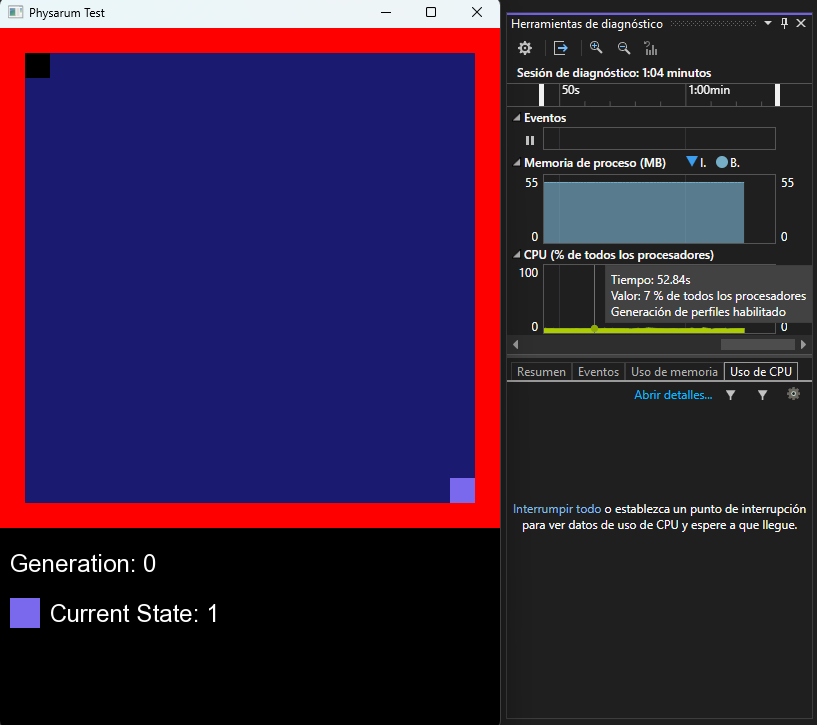
\includegraphics[width=0.5\textwidth]{./images/Pruebas/simulador/image021.png}
        \caption{Rendimiento de la aplicaci\'on con una configuraci\'on inicial en Windows}
        \label{fig:Ruta 7}
    \end{figure}
    %figura 
    \begin{figure}[htbp]
        \centering
        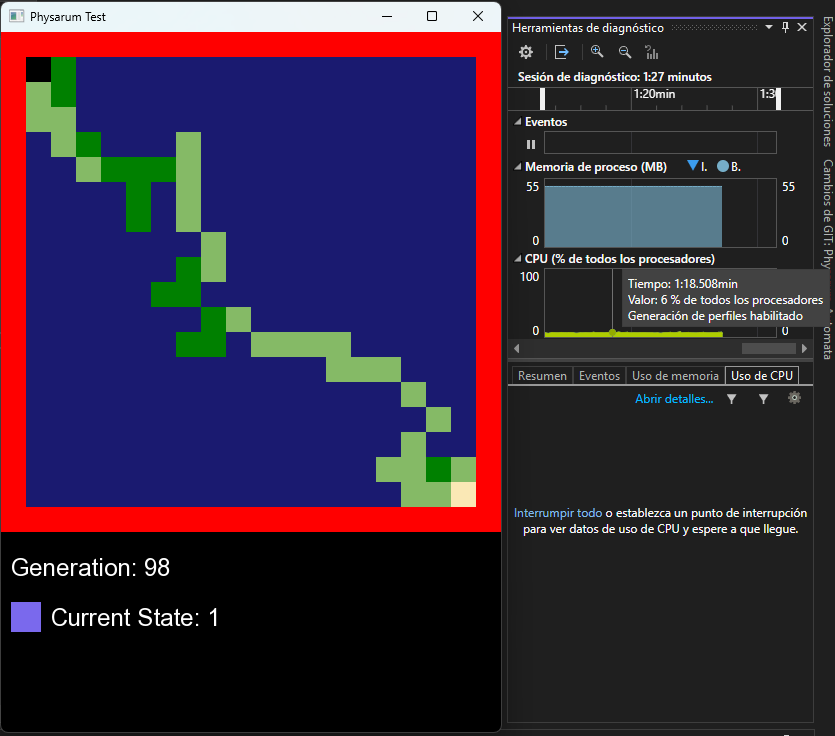
\includegraphics[width=0.5\textwidth]{./images/Pruebas/simulador/image023.png}
        \caption{Rendimiento al obtener la ruta en Windows}
        \label{fig:Ruta 8}
    \end{figure}
    \vskip 0.5cm
    %figura
    \begin{figure}[htbp]
        \centering
        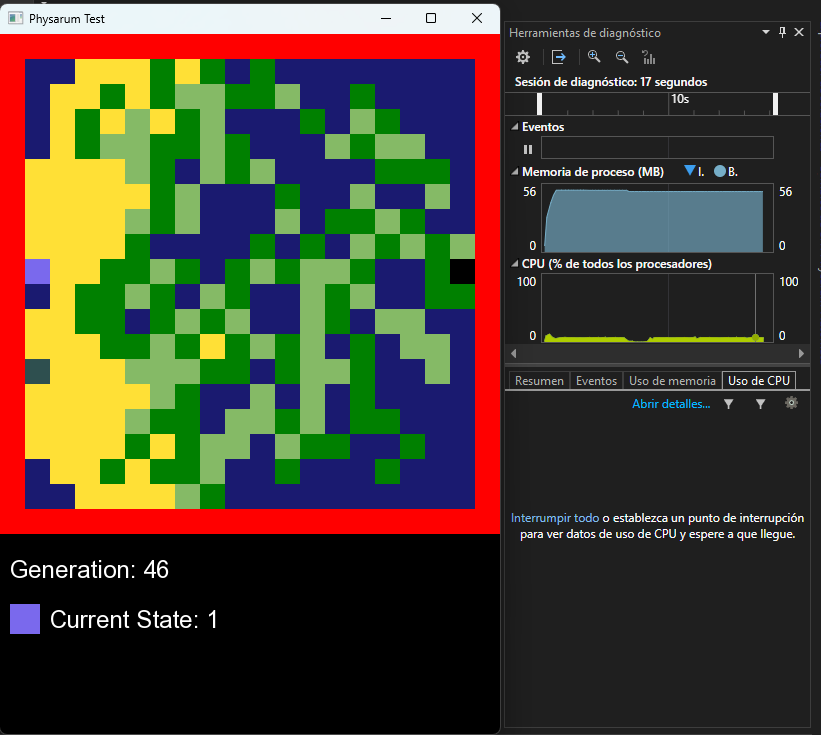
\includegraphics[width=0.5\textwidth]{./images/Pruebas/simulador/image025.png}
        \caption{Rendimiento con configuraci\'on distinta a la anterior mientras se expande en Windows}
        \label{fig:Ruta 9}
    \end{figure}
    \vskip 0.5cm
    %figura
    \begin{figure}[htbp]
        \centering
        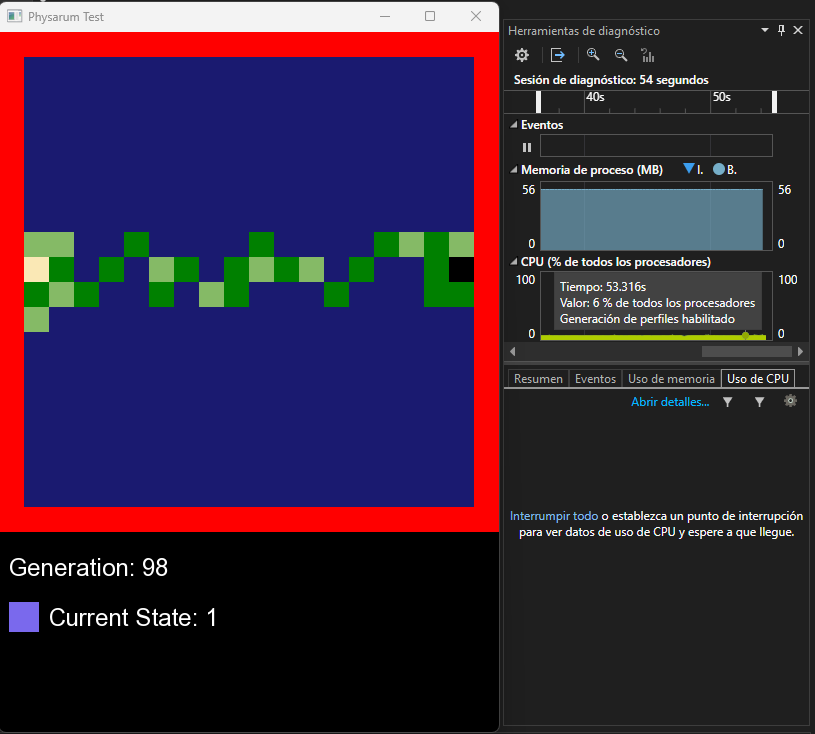
\includegraphics[width=0.5\textwidth]{./images/Pruebas/simulador/image027.png}
        \caption{Rendimiento al obtener una ruta en otra configuraci\'on}
        \label{fig:Ruta 10}
    \end{figure}
    \vskip 0.5cm
    %figura
    \begin{figure}[htbp]
        \centering
        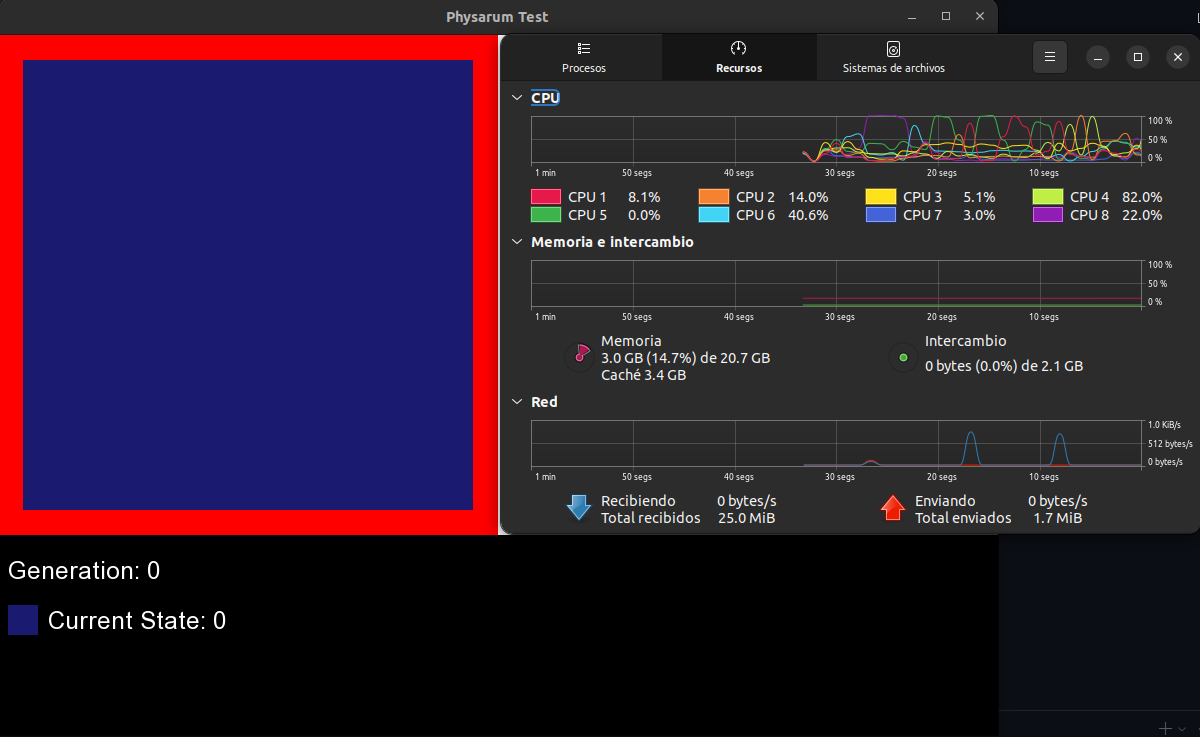
\includegraphics[width=0.5\textwidth]{./images/Pruebas/simulador/image029.png}
        \caption{Rendimiento de la aplicaci\'on al iniciar el programa en Linux}
        \label{fig:Ruta 11}
    \end{figure}
    \vskip 0.5cm
    %figura
    \begin{figure}[htbp]
        \centering
        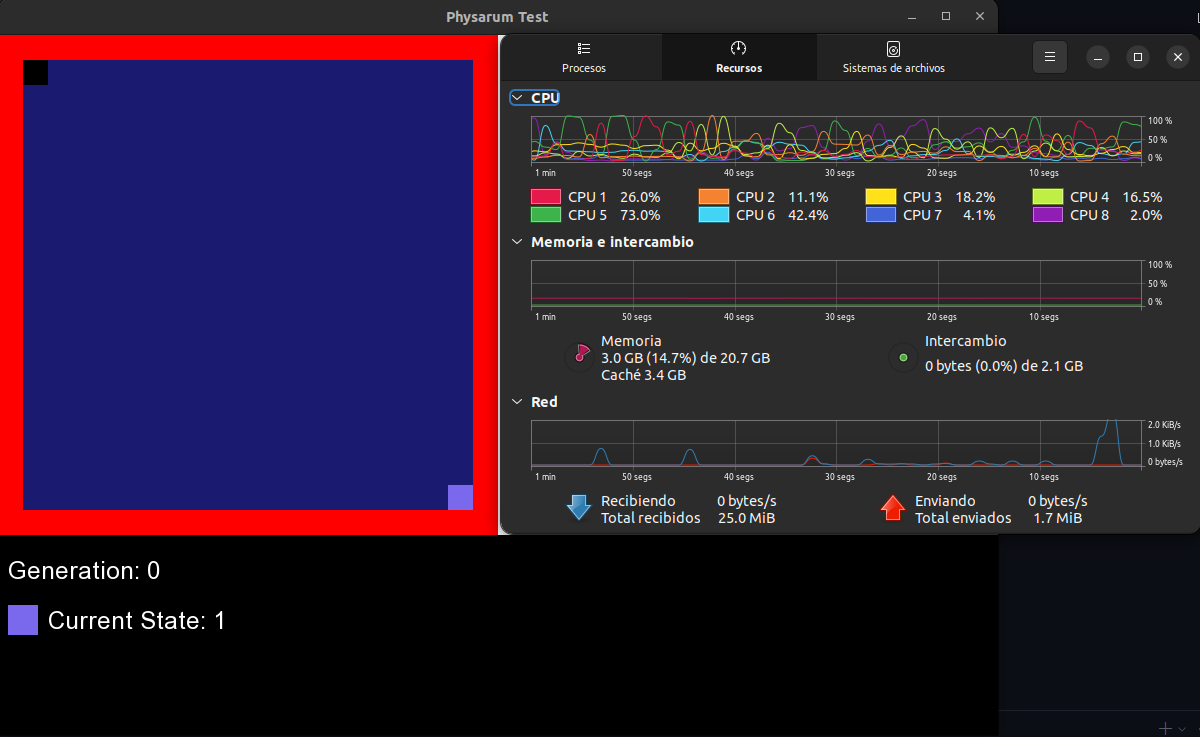
\includegraphics[width=0.5\textwidth]{./images/Pruebas/simulador/image031.png}
        \caption{Rendimiento de la aplicaci\'on con una configuraci\'on inicial en Linux}
        \label{fig:Ruta 12}
    \end{figure}
    \vskip 0.5cm
    %figura
    \begin{figure}[htbp]
        \centering
        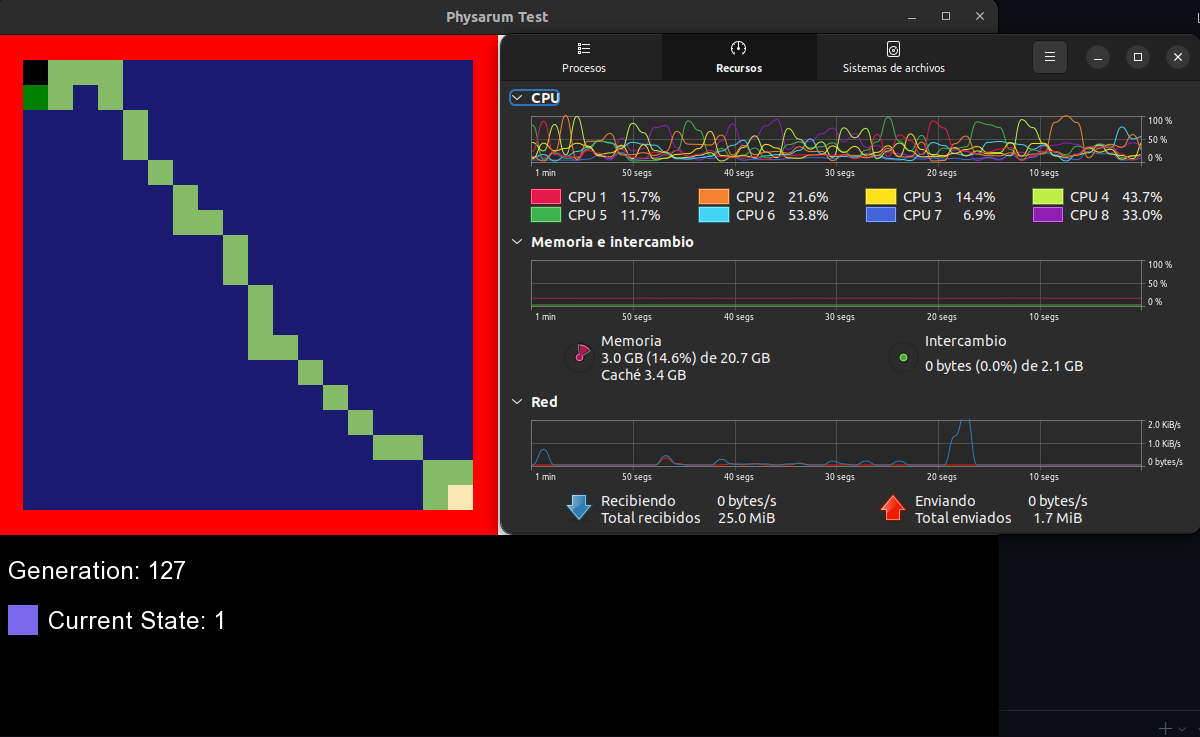
\includegraphics[width=0.5\textwidth]{./images/Pruebas/simulador/image033.png}
        \caption{Rendimiento al obtener la ruta en Linux}
        \label{fig:Ruta 13}
    \end{figure}
    \vskip 0.5cm
    %figura
    \begin{figure}[htbp]
        \centering
        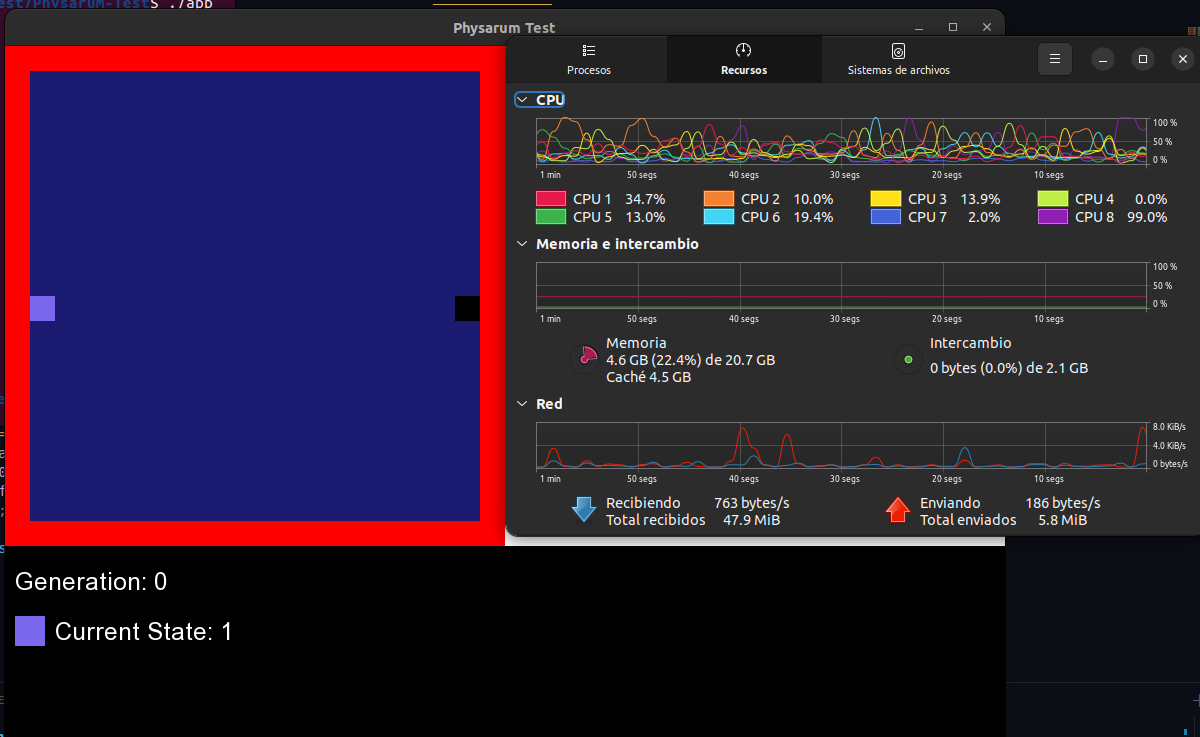
\includegraphics[width=0.5\textwidth]{./images/Pruebas/simulador/image035.png}
        \caption{Rendimiento de la aplicaci\'on con un estado inicial diferente en Linux}
        \label{fig:Ruta 14}
    \end{figure}
    \vskip 0.5cm
    %figura
    \begin{figure}[htbp]
        \centering
        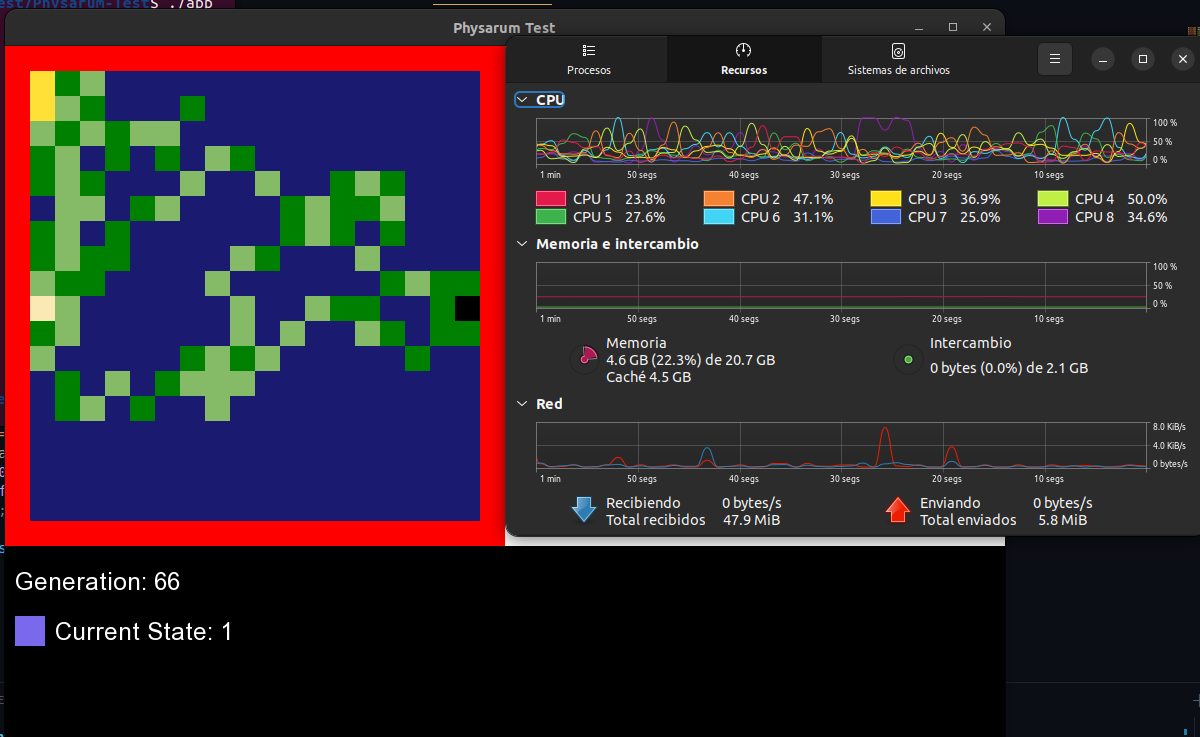
\includegraphics[width=0.5\textwidth]{./images/Pruebas/simulador/image037.png}
        \caption{Rendimiento de la aplicaci\'on durante expansi\'on de Physarum en Linux}
        \label{fig:Ruta 15}
    \end{figure}
    \vskip 0.5cm
    %figura
    \begin{figure}[htbp]
        \centering
        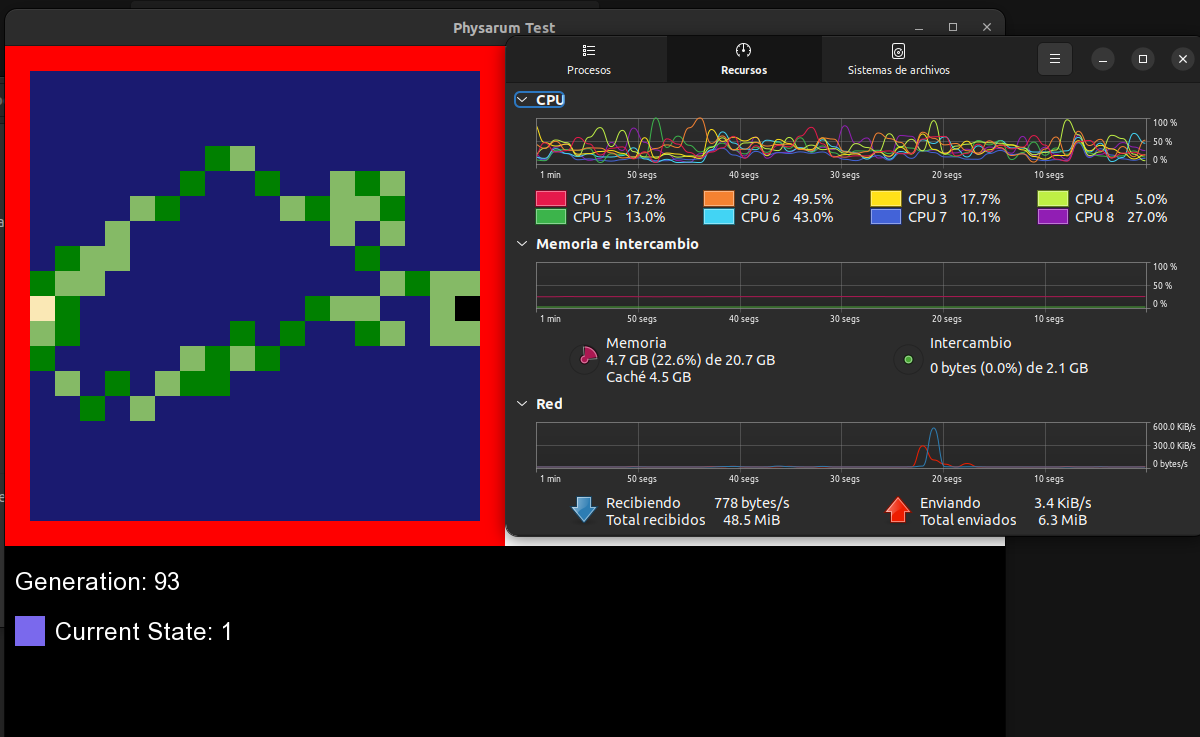
\includegraphics[width=0.5\textwidth]{./images/Pruebas/simulador/image039.png}
        \caption{Rendimiento al obtener una ruta en otra configuraci\'on en Linux}
        \label{fig:Ruta 16}
    \end{figure}
    \vskip 0.5cm
    \clearpage